\section{Aufbereitung der Bilder}
\label{scale_Algos}
OpenFace arbeitet laut Angabe im Paper \cite{OpenFace} am besten auf Gesichtern mit einer Mindestgröße von 100 Pixel, daher werden die Bildbereiche auf diese Größe gebracht. Dies ist notwendig, da die Berechnungen meist auf recht kleinen Bildausschnitten ausgeführt werden muss.\\
Dabei ist es wichtig, dass die Gesichtsmerkmale möglichst gut rekonstruiert werden, um die entsprechenden Landmarks zu bestimmen, dabei erhöht sich der Informationsgehalt der Bilder nicht, sie sind nur besser nutzbar, da sie dem Trainingsdatensatz stärker ähneln.\\
Die von MTCNN gelieferten und vergrößerten Boxen werden auf eine Breite von 130 Pixel gebracht (100 Pixel für den Kopf mit $30\%$ Rand durch Vergrößerung), damit das beinhaltete Gesicht auf der gewünschte Größe dargestellt wird. Neben der Skalierung des Bildausschnittes muss bekannt sein, wie Punkte im skalierten Bildausschnitt in das Frame überführt werden können, damit dies bei späteren Berechnungen berücksichtigt wird.\\
Der Skalierungsfaktor ist für jeden Bildausschnitt individuell und kann sich über die Zeit ändern, wenn sich z.B. die Distanz zwischen Person und Kamera ändert. Von einer zu starken Vergrößerung ist abzuraten, da sich der Rechenaufwand pro Gesicht erhöht und die Zuverlässigkeit der Berechnungen von OpenFace sinkt, z.B. durch Falschdetektion.
\subsection{Bicubic-Skalierung}
Der neue Farbwert wird ermitteln, indem die umliegenden $4\times 4$ Pixelwerte betrachtet werden um den Farbverlauf als eine Funktion 3. Grades zu bestimmen. Somit werden feinere Details besser dargestellt als beim linearen Verfahren und Kanten bleiben eher erhalten. Allerdings kann es durch den bestimmten Verlauf auch zum Überschwingen kommen, wodurch Fehlfarben entstehen können. Ein Beispiel als Ergebnis dieses Verfahrens ist in \autoref{img_Bicubic} zu sehen.\\
\cite{wiki_Bicubic}
\subsection{Lanczos-Skalierung}
Dieser Filter basiert auf einem bewerteten Durchschnitt der umliegenden Pixel um den neuen Pixelwert zu erhalten. Die Bewertung der einzelnen Pixel wird durch eine Sinc-Funktion bestimmt, damit weiter entferntere Pixel schwächer bewertet werden als näher liegende, siehe \autoref{img_Lanczos}.\\
Außerdem wird durch den Kurvenverlauf der Bewertungsfunktion eine gewisse Bildschärfe erreicht. Die Funktion kann und wird für die Anwendung auf einen $8\times 8$ Pixel großen Bereich begrenzt.\\
\cite{wiki_Lanczos}
\[ L(x)= \left\{ \begin{array}{ll}
\frac{\sin(\pi x)}{\pi x} \cdot \frac{\sin(\pi \frac{x}{a})}{\pi \frac{x}{a}} & \textrm{wenn } -a < x <a, a\ne 0\\
1 & \textrm{wenn } x = 0\\
0 & \textrm{sonst}
\end{array}\right. \]
\subsection{Linear-Skalierung}
Um den neuen Farbwert zu ermitteln, wird zwischen den nächstgelegenen umliegenden Pixel linear Interpoliert, wodurch weitere Farbwerte entstehen. Das Ergebnis ist gleichmäßiger als Neares Neighbor, und dennoch ein recht einfaches Verfahren. Die Kanten wirken allerdings unscharf, siehe \autoref{img_Linear}.
\subsection{Nearest-Neighbor-Skalierung}
Dieses Verfahren verwendet als neuer Farbwert, den gleichen Wert wie das nächstgelegene Pixel. Dadurch werden nur die ehemaligen Pixel größer und das Gesicht wirkt sehr Kantig, da keine neuen Farbwerte bestimmt werden, siehe \autoref{img_NN}. Bei der Vergrößerung des Schachbretts sind kein Farbfehler aufgetreten, da nur zwei Farben vorhanden und Positionsabhängig sind.
\begin{figure}
	\centering
	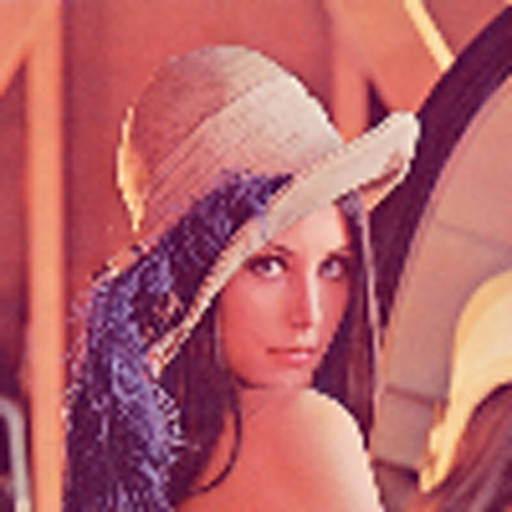
\includegraphics[width=0.2\linewidth]{img/lena100_CUBIC}
	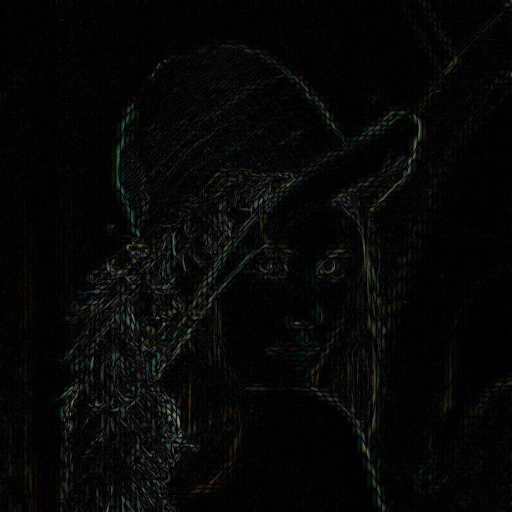
\includegraphics[width=0.2\linewidth]{img/lena100_CUBIC_differenz}
	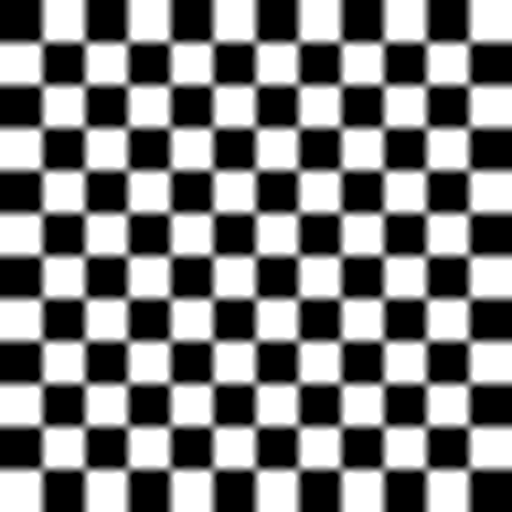
\includegraphics[width=0.2\linewidth]{img/Schachbrett_CUBIC}
	\caption{Die ursprüngliche Abbildung von Lena betrug 100 Pixel Kantenlänge und beim Schachbrett 48 Pixel, beide wurden mittels bikubischem Verfahren auf 512 Pixel vergrößert und bei Lena die Differenz zum originalen Lena-Bild bestimmt, siehe mittleres Bild}
	\label{img_Bicubic}
\end{figure}
\begin{figure}
	\centering
	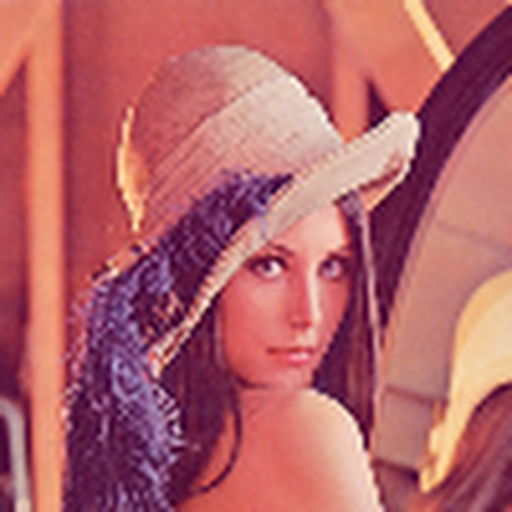
\includegraphics[width=0.2\linewidth]{img/lena100_LANCZOS4}
	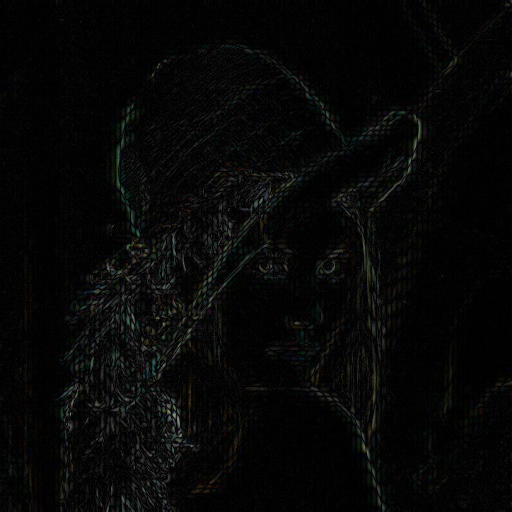
\includegraphics[width=0.2\linewidth]{img/lena100_LANCZOS4_differenz}
	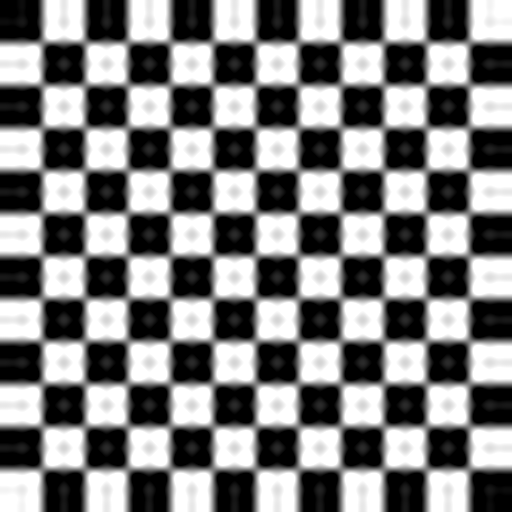
\includegraphics[width=0.2\linewidth]{img/Schachbrett_LANCZOS4}
	\caption{Die ursprüngliche Abbildung von Lena betrug 100 Pixel Kantenlänge und beim Schachbrett 48 Pixel, beide wurden mittels Lanczus-Verfahren auf 512 Pixel vergrößert und bei Lena die Differenz  zum originalen Lena-Bild bestimmt, siehe mittleres Bild}
	\label{img_Lanczos}
\end{figure}
\begin{figure}
	\centering
	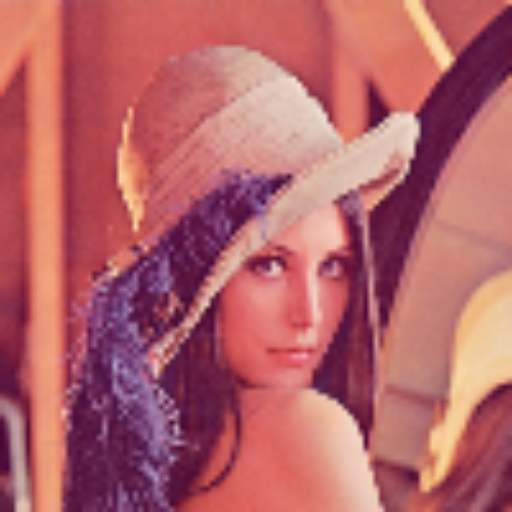
\includegraphics[width=0.2\linewidth]{img/lena100_LINEAR}
	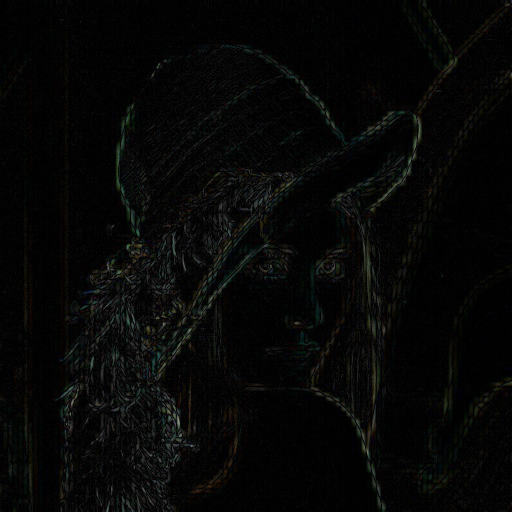
\includegraphics[width=0.2\linewidth]{img/lena100_LINEAR_differenz}
	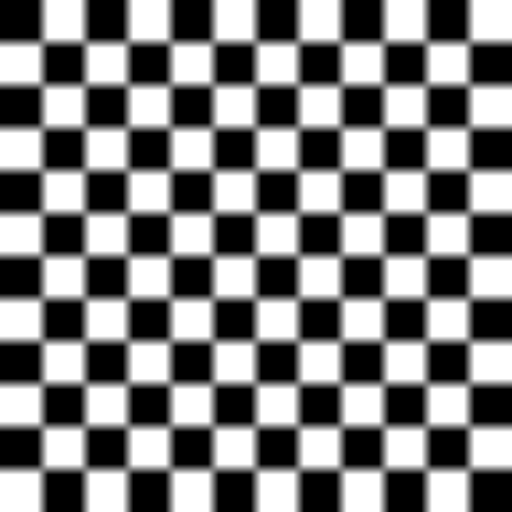
\includegraphics[width=0.2\linewidth]{img/Schachbrett_LINEAR}
	\caption{Die ursprüngliche Abbildung von Lena betrug 100 Pixel Kantenlänge und beim Schachbrett 48 Pixel, beide wurden mittels linearer Interpolation auf 512 Pixel vergrößert und bei Lena die Differenz zum originalen Lena-Bild bestimmt, siehe mittleres Bild}
	\label{img_Linear}
\end{figure}
\begin{figure}
	\centering
	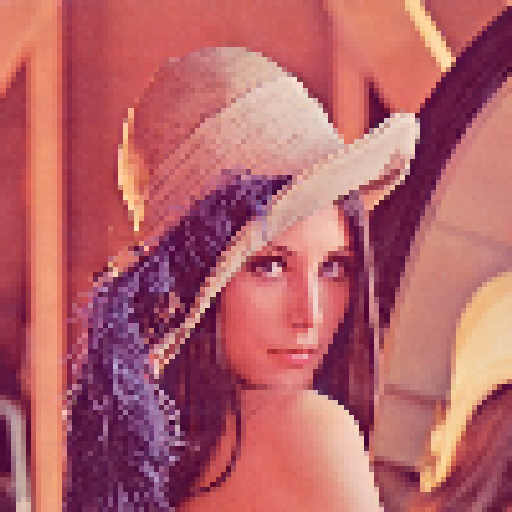
\includegraphics[width=0.2\linewidth]{img/lena100_NN}
	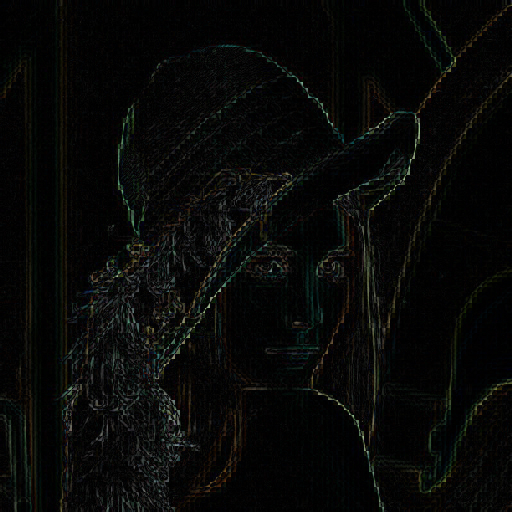
\includegraphics[width=0.2\linewidth]{img/lena100_NN_differenz}
	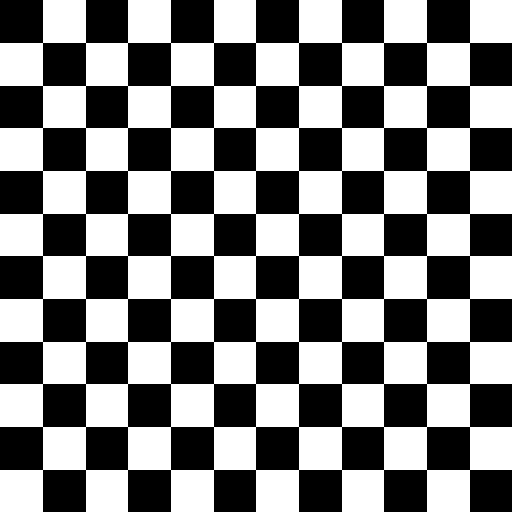
\includegraphics[width=0.2\linewidth]{img/Schachbrett_NN}
	\caption{Die ursprüngliche Abbildung von Lena betrug 100 Pixel Kantenlänge und beim Schachbrett 48 Pixel, beide wurden mittels Nearest-Neighbor auf 512 Pixel vergrößert und bei Lena die Differenz zum originalen Lena-Bild bestimmt, siehe mittleres Bild}
	\label{img_NN}
\end{figure}
% http://docs.opencv.org/2.4/modules/imgproc/doc/geometric_transformations.html#resize